\chapter{Practical aspects of DFT}
\label{sec:Practical DFT}

\section{The Exchange-Correlation functional}
From the former section, we know that the one peace of information missing of the density functional theory is the complex exchange-correlation energy $E_{\text{xc}}[n]$ that must account for all the simplifications and approximations employed in Kohn-Sham DFT. In this section we will explore some of the commonly used approximations to exchange-correlation functional. In this project we limit ourselves to 4 levels of complexity, first is the local density approximation (LDA), followed by the generalized gradient approximation (GGA). These two are the least complex and computationally affordable methods. Next is the methods such as meta-GGA implementations and finally the very accurate, but equally demanding hybrid-functionals. In addition, we have methods such as DFT+U, the Minnesota functionals, and double hybrids plus more, but these are outside the scope of this project.  

\subsection{Local density approximation}
A homogeneous electron gas (HEG) is the sole case we know of where the exchange-correlation functional can be determined exactly, because in this simple case the electron density is constant. The LDA works by setting the exchange-correlation potential $V_\text{XC}(\boldsymbol{r})$ at every position equal to that of the homogeneous electron gas, ie

\begin{equation}
V_\text{XC}(\boldsymbol{r}) = V_\text{XC} ^\text{HEG}[n(\boldsymbol{r})] .
\end{equation} 

Obviously the LDA is of limited use given that a large part of what makes materials interesting is the variation in the electronic density. In the case of limitations LDA is for example known to overestimate binding energies and  underestimate the band gap in semiconductors and insulators. On the other hand, LDA provide generally adequate results in bulk materials with slowly varying charge density, for example equilibrium distances and vibrational frequencies. The biggest upside of LDA however comes from the low computational cost, and was one of the first big success-stories of DFT. 


\subsection{Generalized gradient approximation}
A natural succession to the local density approximation is the family of generalized gradient approximation (GGA) that also include the gradient of the electron density

\begin{equation}
V_\text{XC} ^\text{GGA} (\boldsymbol{r}) = V_\text{XC} [n(\boldsymbol{r}), \nabla n(\boldsymbol{r})].
\end{equation}

The way one can implement the gradient are plenty-full and complicated. Two of the most common methods are the Perdew-Wang 91 (PW91) \cite{pw91} and the Perdew-Burke-Ernzerhof (PBE) GGA \cite{pbe}. This project will utilize the latter, which came to fruition in  1996 in an article by Perdew, Burke and Ernzerhof appropriately named "Generalized Gradient Approximation Made Simple". The key point regarding the PBE functional is that it's a non-empirical method thus providing reliable and adequate accuracy over a wide range of systems, as compared to for instance the BLYP functional that provide excellent accuracy of organic molecules but fails in other cases \cite{PBE_forum}. 

\subsection{Meta-GGA}   
Meta-GGA functionals is the final level of  complexity of the non-emperical approximations to the exchange-correlation functional. In addition to the the constant density (LDA) and local gradient of the density (GGA), meta-GGA methods consider the kinetic energy density of the occupied Kohn-Sham orbitals \cite{metagga}
 
\begin{equation}
	\tau_\omega = \sum_i ^\text{occ}\frac{1}{2}|\nabla_{\psi_{i, \omega}}|^2.
\end{equation}

The role of this quantity on the the calculated band gap is well described in \cite{xc_kineticEnergy}. In this project we employ a meta-GGA functional named \textit{Strongly Constrained Appropriately Normed}, or SCAN. This functional is the only known functional to satisfy all 17 known exact constraints of the XC functional \cite{scan}. The SCAN functional have found evidence of particularly superior accuracy of energies and geometries especially in diversly bonded structures  \cite{scan_divbond}, and some indication of improved band gaps and density of states over GGA and LDA functionals \cite{scan_pbe}. However delivers overall less accurate band gaps compared to other meta-GGA functionals such as the \textit{modified Becke-Johnson} \cite{mbj}. Unfortunately, MBJ proved too difficult to converge for the particular materials in this project and we instead opt for SCAN. 
\begin{figure}[H]
\centering
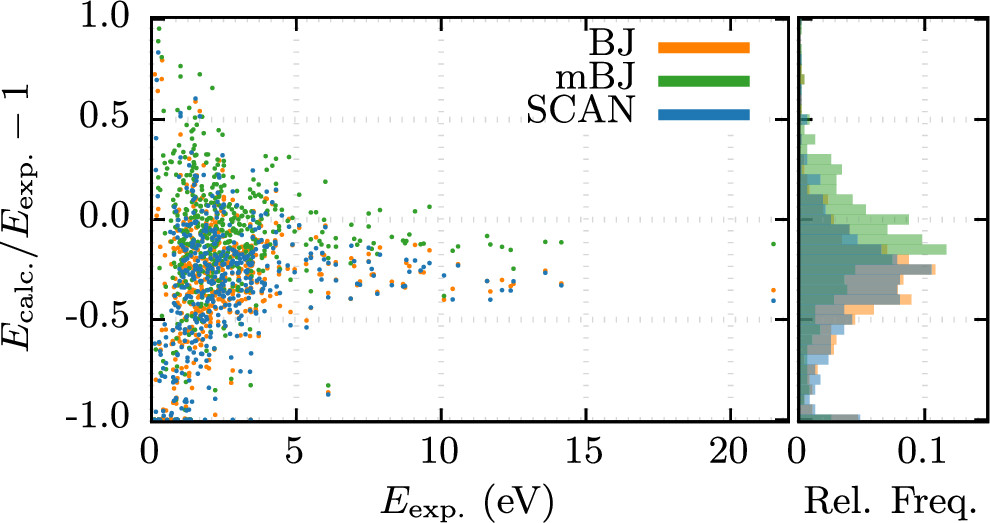
\includegraphics[scale=0.3]{method/dft/metagga.jpeg}
\caption{Calculated to experimental band gap measurements of Becke-Johnsoon, modified Becke-Johnson and SCAN functionals \cite{xc_benchmark}}
\end{figure}

\subsection{Hybrid functionals}

The most accurate functional we employ in this project belong to the family of \textit{hybrid functionals}. Accordingly this method consist of a hybrids between simpler functionals such as LDA, PBE or even meta-GGA and the exact treatment of exchange energy from Hartree-Fock, for example the global hybrid functional PBE0 \cite{pbe0} described as

\begin{equation}
E_\text{xc} ^\text{PBE0} = (1-\alpha)E_x ^\text{PBE} + \alpha E_x ^{HF} + E_c ^{PBE}, 
\end{equation}

 where $\alpha$ is the mixing parameter to decide the balance between the exchange energy, denoted $x$ of Hartree-Fock with PBE. Alike the last term represent the correlation energy from the PBE functional. This parameter alpha is determined empirically, thus making hybrid functional a semi-empirical model. Obviously considering the exact exchange in Hartree-Fock is a computationally challenging prospect. Heyd-Scuseria-Ernzerhof managed to lower the cost by the concept of Screened functionals that separate the Coloumb interaction into long-range and short-range interaction by a function $erfc(\mu r)$. These are known as HSE functionals \cite{hse}, one of the superior methods for accurate band gaps is the HSE06 hybrid functional \cite{hse06}, with $\alpha = 0.25$ and $\mu = 0.11$.  
 
\subsection{Outlook} 
 
In many cases LDA and GGA suffice, PBE especially is by most considered the conventional standard for DFT calculations, for its balance of accuracy, cost and wide range applicability. However, distinctly concerning the band gap of a solids, both of these fall short. This is because the band gap of DFT calculations is complicated by the fact that the derivative of the XC-functional is discontinues with respect to the electron concentration \cite{xc_derivative}, thus the simpler functionals fail to recall the experimental values since the total band gap in DFT is the fundamental gap (valence - conduction) + this contribution. This is corrected in meta-GGA and hybrid functionals in the generalized Kohn-Sham scheme. Lastly, we would like to refer the reader to the work of Borlido, Aull, Huran, Tran, Marques, and Botti whom in 2019 conducted an exhastive investigation of the band gap of over 470 uniqe non-magnetic compounds in order to benchmark the relative performance of several of the available and wideley used XC-functionals \cite{xc_benchmark}. In this large-scale project they found overwhelming confirmation that the HSE06 functional followed closely by Modified-Becke Johnson is the superior choice for accurate band-gap measures. Regarding the SCAN functional, in several cases this yielded outputs very comparable to MBJ, and produce much better formation energies than PBE, but tends to overstimate in magnetic alloys. On the other side both LDA and PBE resulted in $50\%$ and $30\%$ under-estimation of the band gap or in several cases miss-classified compounds as metals, this was particularly evident in materials containing Ni and other 3d elements.  
 

\section{Plane waves and reciprocal space}

The solution of the Shr\"{o}dinger equation for a free electron have a simple analytic solution $\psi_k = Ae^{i\boldsymbol{k}\boldsymbol{r}}$. In a crystalline matter with a periodic potential $V(\boldsymbol{r}) = V(\boldsymbol{r} + \boldsymbol{R})$, the single-electron wavefunction takes the form 

\begin{equation}
\psi_{\boldsymbol{k}}(\boldsymbol{r}) = u_{\boldsymbol{k}}(\boldsymbol{r})e^{i\boldsymbol{k}\boldsymbol{r}},    
\end{equation}

where $u_{\boldsymbol{k}}(\boldsymbol{r})$ is a Bloch wave with the periodicity of the crystal and $e^{ikr}$ is called a plane wave. Because we use plane waves, DFT calculations are often referred to as plane wave calculations. The Bloch wave is the sum of all plane waves with wave vector equal to the reciprocal wave vector $\boldsymbol{G}$, described as 

\begin{equation}
    u_{\boldsymbol{k}}(\boldsymbol{r}) = \sum_{\boldsymbol{G}} c_{\boldsymbol{G}}e^{i\boldsymbol{G}\boldsymbol{r}},
\end{equation}
 which gives us the final expression for $\psi_k (\boldsymbol{r})$ 
 
\begin{equation}
    \psi_{\boldsymbol{k}}(\boldsymbol{r}) = \sum_{\boldsymbol{G}} c_{\boldsymbol{k} + \boldsymbol{G}}e^{i(\boldsymbol{k} + \boldsymbol{G})\boldsymbol{r}}
\end{equation}

Clearly, the infinite summation over all $\boldsymbol{G}$ necessary to evaluate the wavefunction at a single point in reciprocal space is computationally unfeasible. In order to reduce this computational burden, we can introduce a maximum cutoff value of the energy $E_{\text{cut}}$. This is possible because equation 5.7 is the solution of the Shr\"{o}dinger equation with corresponding kinetic energy 

\begin{equation}
    E = \frac{\hbar^2}{2m}|\boldsymbol{k} + \boldsymbol{G}|^2.
\end{equation}

Assuming that the lower energy solutions are the most interesting, we can limit the calculations to plane waves with energy less than $E_{\text{cut}}$ as
\begin{equation}
    E_{\text{cut}} = \frac{\hbar^2}{2m}G_{\text{cut}}.
\end{equation}

Thus, we can reduce the infinitely large sum above to a much more feasible calculation
\begin{equation}
    \psi_{\boldsymbol{k}}(\boldsymbol{r}) = \sum_{|\boldsymbol{k} + \boldsymbol{G}| < G_{\text{cut}}} u_{\boldsymbol{k} + \boldsymbol{G}}(\boldsymbol{r})e^{i(\boldsymbol{k} + \boldsymbol{G})\boldsymbol{r}}.
\end{equation}

The cutoff energy is determined by performing a number of calculations of different cutoff and observe the convergence with respect to the total energy of the system. Another important parameter to specify in DFT calculations is the number of k-points. As seen in the above expression the wavevector $k$ plays a big role in DFT, an other case that is more convinient to calculate in k-space is integrals of the from 
\begin{equation}
    g = \frac{V_{\text{cell}}}{(2\pi)^3} \int_{\text{BZ}} g(\boldsymbol{k})d\boldsymbol{k},
\end{equation}
for instance the density of states. Note that "BZ" indicate that the integral is evaluated for all $\boldsymbol{k}$ in the Brillouin zone. This integral can be approximated by evaluating it at a set of discrete k-points in reciprocal space and summing over the points with appropriately assigned weights. A larger set of points leads to more exact approximations. The method for selecting k-points in reciprocal space was developed by Monkhorst and Pack in 1976, where one specify a number of points in each dimension $N x N x N$. Recalling that reciprocal space is inverse to regular space, supercells with equal and large dimensions converge at smaller values of N, and inversly for cells of small dimsion. The total number of k-points required for accurate can be reduced by utulizing the symmetry of the cell, in which we can exactly approximate the entire BZ by extending a lesser zone through symmetry of the crystal lattice. This reduced zone is named the irreducible Brillouin zone (IBZ). 

The required number of k-points for a given calculation can be found alike the cutoff energy by performing convergence tests with respect to the total energy of the system. Metals in particular require a large number of k-points because of discontinues integrals in the Brillouin zone around the Fermi surface where the states discontinuously change from occupied to non-occupied. To reduce the cost of this operation, there are two primary methods, tetrhaedon and smearing. The idea behind the tetrahedon method is to use the discrete set of k-points to fill the reciprocal space with tethraeda and interpolate the function within each tethraeda such that the function can be integrated in the entire space rather than at discrete points. The latter approach for solving discontinuos integrals is to smear out the discontinuity and thus transforming the integral to a continuous one. A good analogy to this method is the fermi-dirac function, in which a small variable $\sigma$ transform a step-function into a continuous function that can be integrated by standard methods.

A final consideration to how DFT is applied in practice is how the core electrons are handled. Tightly bound core electrons as opposed to valence electrons demand a greater number of plane-waves to converge. The most efficient method of reducing the expenses of core-electrons are so-called pseudopotentials. This method works by approximating the electron density of the core electrons by a constant density that mimic the properties of true ion core and core electrons. This density is then remained constant for all subsequent calculations, in other words only considering the valence electrons while regarding the core electrons as frozen-in. There are currently two popular types of psudopotentials used in DFT, so-called ultrasoft psudopotentials (USPPs) developed by Vanderbilt, and the projector augmented-wave (PAW) method by Bloch \cite{PAW1}, \cite{PAW2}.

\section{Self-consistent field calculation}

\begin{figure}[H]
\centering
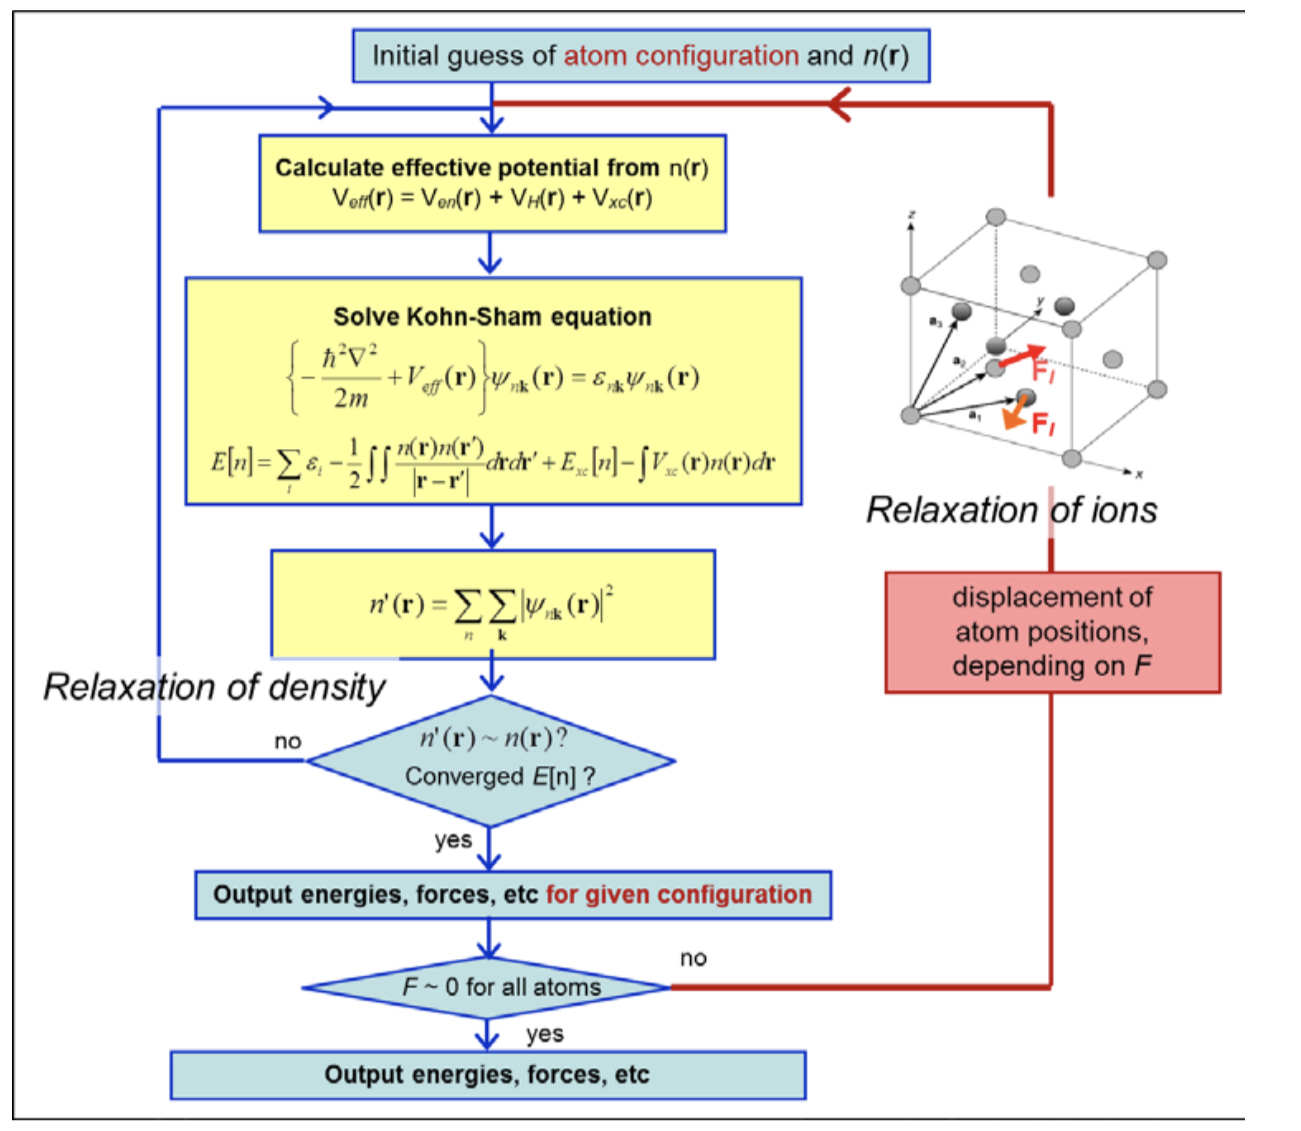
\includegraphics[width=\textwidth]{theory/selfConsistentDFT.jpeg}
\caption{Self consistent iteration of a DFT calculation. Figure adopted from lecture notes fys-mena4111 \cite{persson2020}}
\end{figure}

Preluding this section, we have considered the fundamental theory of DFT and it's practical ability to model various materials. Figure 5.2 illustrate the self-consistent field calculation scheme for how DFT calculations are performed in practice. The initial problem posed by DFT is that all properties rely on the density, and are following dependent on each other. For instance, the effective potential is dependent on the density, which again is dependent on the eigenfunctions, that rely on the effective potential again. The cleaver approach begin with an initial guess to the density from which we can solve the Kohn-Sham equation and obtain the corresponding eigenfunctions. Following is an iterative method where we apply the recently calculated eigenfunctions to determine a new density and repeat the procedure above. This is repeated until the total energy is converged, by an own-defined criterion. Equivalently, the optimal ionic positions can be found by a similar approach. This method is based on quasi-Newton algorithms to minimize the forces between ions. 



